\chapter{Memory Visualization}
\label{app:memory}

\begin{figure}
    \centering
    %% Creator: Matplotlib, PGF backend
%%
%% To include the figure in your LaTeX document, write
%%   \input{<filename>.pgf}
%%
%% Make sure the required packages are loaded in your preamble
%%   \usepackage{pgf}
%%
%% Also ensure that all the required font packages are loaded; for instance,
%% the lmodern package is sometimes necessary when using math font.
%%   \usepackage{lmodern}
%%
%% Figures using additional raster images can only be included by \input if
%% they are in the same directory as the main LaTeX file. For loading figures
%% from other directories you can use the `import` package
%%   \usepackage{import}
%%
%% and then include the figures with
%%   \import{<path to file>}{<filename>.pgf}
%%
%% Matplotlib used the following preamble
%%   \usepackage{fontspec}
%%   \setmainfont{DejaVuSerif.ttf}[Path=\detokenize{/usr/lib/python3.10/site-packages/matplotlib/mpl-data/fonts/ttf/}]
%%   \setsansfont{DejaVuSans.ttf}[Path=\detokenize{/usr/lib/python3.10/site-packages/matplotlib/mpl-data/fonts/ttf/}]
%%   \setmonofont{DejaVuSansMono.ttf}[Path=\detokenize{/usr/lib/python3.10/site-packages/matplotlib/mpl-data/fonts/ttf/}]
%%
\begingroup%
\makeatletter%
\begin{pgfpicture}%
\pgfpathrectangle{\pgfpointorigin}{\pgfqpoint{5.545496in}{3.007709in}}%
\pgfusepath{use as bounding box, clip}%
\begin{pgfscope}%
\pgfsetbuttcap%
\pgfsetmiterjoin%
\definecolor{currentfill}{rgb}{1.000000,1.000000,1.000000}%
\pgfsetfillcolor{currentfill}%
\pgfsetlinewidth{0.000000pt}%
\definecolor{currentstroke}{rgb}{1.000000,1.000000,1.000000}%
\pgfsetstrokecolor{currentstroke}%
\pgfsetstrokeopacity{0.000000}%
\pgfsetdash{}{0pt}%
\pgfpathmoveto{\pgfqpoint{0.000000in}{0.000000in}}%
\pgfpathlineto{\pgfqpoint{5.545496in}{0.000000in}}%
\pgfpathlineto{\pgfqpoint{5.545496in}{3.007709in}}%
\pgfpathlineto{\pgfqpoint{0.000000in}{3.007709in}}%
\pgfpathlineto{\pgfqpoint{0.000000in}{0.000000in}}%
\pgfpathclose%
\pgfusepath{fill}%
\end{pgfscope}%
\begin{pgfscope}%
\pgfsetbuttcap%
\pgfsetmiterjoin%
\definecolor{currentfill}{rgb}{1.000000,1.000000,1.000000}%
\pgfsetfillcolor{currentfill}%
\pgfsetlinewidth{0.000000pt}%
\definecolor{currentstroke}{rgb}{0.000000,0.000000,0.000000}%
\pgfsetstrokecolor{currentstroke}%
\pgfsetstrokeopacity{0.000000}%
\pgfsetdash{}{0pt}%
\pgfpathmoveto{\pgfqpoint{0.183333in}{0.183333in}}%
\pgfpathlineto{\pgfqpoint{2.697748in}{0.183333in}}%
\pgfpathlineto{\pgfqpoint{2.697748in}{2.697748in}}%
\pgfpathlineto{\pgfqpoint{0.183333in}{2.697748in}}%
\pgfpathlineto{\pgfqpoint{0.183333in}{0.183333in}}%
\pgfpathclose%
\pgfusepath{fill}%
\end{pgfscope}%
\begin{pgfscope}%
\pgfpathrectangle{\pgfqpoint{0.183333in}{0.183333in}}{\pgfqpoint{2.514415in}{2.514415in}}%
\pgfusepath{clip}%
\pgfsys@transformshift{0.183333in}{0.183333in}%
\pgftext[left,bottom]{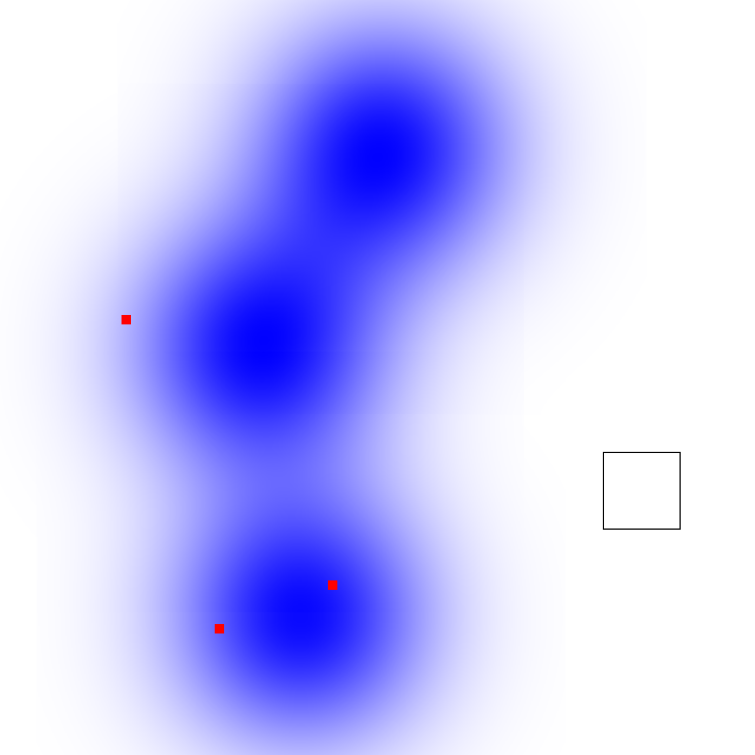
\includegraphics[interpolate=true,width=2.516667in,height=2.516667in]{memory-img0.png}}%
\end{pgfscope}%
\begin{pgfscope}%
\pgfsetrectcap%
\pgfsetmiterjoin%
\pgfsetlinewidth{1.254687pt}%
\definecolor{currentstroke}{rgb}{0.150000,0.150000,0.150000}%
\pgfsetstrokecolor{currentstroke}%
\pgfsetdash{}{0pt}%
\pgfpathmoveto{\pgfqpoint{0.183333in}{0.183333in}}%
\pgfpathlineto{\pgfqpoint{0.183333in}{2.697748in}}%
\pgfusepath{stroke}%
\end{pgfscope}%
\begin{pgfscope}%
\pgfsetrectcap%
\pgfsetmiterjoin%
\pgfsetlinewidth{1.254687pt}%
\definecolor{currentstroke}{rgb}{0.150000,0.150000,0.150000}%
\pgfsetstrokecolor{currentstroke}%
\pgfsetdash{}{0pt}%
\pgfpathmoveto{\pgfqpoint{2.697748in}{0.183333in}}%
\pgfpathlineto{\pgfqpoint{2.697748in}{2.697748in}}%
\pgfusepath{stroke}%
\end{pgfscope}%
\begin{pgfscope}%
\pgfsetrectcap%
\pgfsetmiterjoin%
\pgfsetlinewidth{1.254687pt}%
\definecolor{currentstroke}{rgb}{0.150000,0.150000,0.150000}%
\pgfsetstrokecolor{currentstroke}%
\pgfsetdash{}{0pt}%
\pgfpathmoveto{\pgfqpoint{0.183333in}{0.183333in}}%
\pgfpathlineto{\pgfqpoint{2.697748in}{0.183333in}}%
\pgfusepath{stroke}%
\end{pgfscope}%
\begin{pgfscope}%
\pgfsetrectcap%
\pgfsetmiterjoin%
\pgfsetlinewidth{1.254687pt}%
\definecolor{currentstroke}{rgb}{0.150000,0.150000,0.150000}%
\pgfsetstrokecolor{currentstroke}%
\pgfsetdash{}{0pt}%
\pgfpathmoveto{\pgfqpoint{0.183333in}{2.697748in}}%
\pgfpathlineto{\pgfqpoint{2.697748in}{2.697748in}}%
\pgfusepath{stroke}%
\end{pgfscope}%
\begin{pgfscope}%
\definecolor{textcolor}{rgb}{0.150000,0.150000,0.150000}%
\pgfsetstrokecolor{textcolor}%
\pgfsetfillcolor{textcolor}%
\pgftext[x=1.440541in,y=2.781081in,,base]{\color{textcolor}\rmfamily\fontsize{12.000000}{14.400000}\selectfont \(\displaystyle t = 9\)}%
\end{pgfscope}%
\begin{pgfscope}%
\pgfsetbuttcap%
\pgfsetmiterjoin%
\definecolor{currentfill}{rgb}{1.000000,1.000000,1.000000}%
\pgfsetfillcolor{currentfill}%
\pgfsetlinewidth{0.000000pt}%
\definecolor{currentstroke}{rgb}{0.000000,0.000000,0.000000}%
\pgfsetstrokecolor{currentstroke}%
\pgfsetstrokeopacity{0.000000}%
\pgfsetdash{}{0pt}%
\pgfpathmoveto{\pgfqpoint{2.931081in}{0.183333in}}%
\pgfpathlineto{\pgfqpoint{5.445496in}{0.183333in}}%
\pgfpathlineto{\pgfqpoint{5.445496in}{2.697748in}}%
\pgfpathlineto{\pgfqpoint{2.931081in}{2.697748in}}%
\pgfpathlineto{\pgfqpoint{2.931081in}{0.183333in}}%
\pgfpathclose%
\pgfusepath{fill}%
\end{pgfscope}%
\begin{pgfscope}%
\pgfpathrectangle{\pgfqpoint{2.931081in}{0.183333in}}{\pgfqpoint{2.514415in}{2.514415in}}%
\pgfusepath{clip}%
\pgfsys@transformshift{2.931081in}{0.183333in}%
\pgftext[left,bottom]{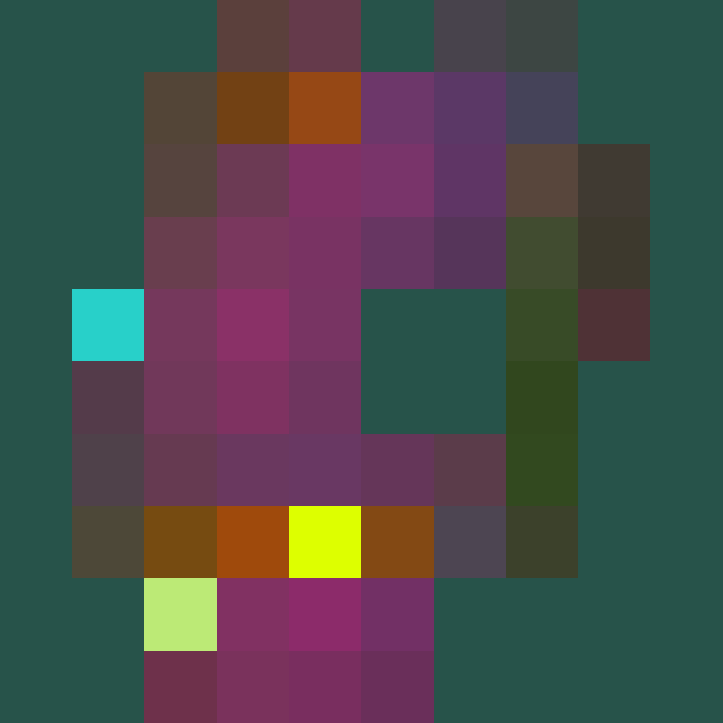
\includegraphics[interpolate=true,width=2.516667in,height=2.516667in]{memory-img1.png}}%
\end{pgfscope}%
\begin{pgfscope}%
\pgfsetrectcap%
\pgfsetmiterjoin%
\pgfsetlinewidth{1.254687pt}%
\definecolor{currentstroke}{rgb}{0.150000,0.150000,0.150000}%
\pgfsetstrokecolor{currentstroke}%
\pgfsetdash{}{0pt}%
\pgfpathmoveto{\pgfqpoint{2.931081in}{0.183333in}}%
\pgfpathlineto{\pgfqpoint{2.931081in}{2.697748in}}%
\pgfusepath{stroke}%
\end{pgfscope}%
\begin{pgfscope}%
\pgfsetrectcap%
\pgfsetmiterjoin%
\pgfsetlinewidth{1.254687pt}%
\definecolor{currentstroke}{rgb}{0.150000,0.150000,0.150000}%
\pgfsetstrokecolor{currentstroke}%
\pgfsetdash{}{0pt}%
\pgfpathmoveto{\pgfqpoint{5.445496in}{0.183333in}}%
\pgfpathlineto{\pgfqpoint{5.445496in}{2.697748in}}%
\pgfusepath{stroke}%
\end{pgfscope}%
\begin{pgfscope}%
\pgfsetrectcap%
\pgfsetmiterjoin%
\pgfsetlinewidth{1.254687pt}%
\definecolor{currentstroke}{rgb}{0.150000,0.150000,0.150000}%
\pgfsetstrokecolor{currentstroke}%
\pgfsetdash{}{0pt}%
\pgfpathmoveto{\pgfqpoint{2.931081in}{0.183333in}}%
\pgfpathlineto{\pgfqpoint{5.445496in}{0.183333in}}%
\pgfusepath{stroke}%
\end{pgfscope}%
\begin{pgfscope}%
\pgfsetrectcap%
\pgfsetmiterjoin%
\pgfsetlinewidth{1.254687pt}%
\definecolor{currentstroke}{rgb}{0.150000,0.150000,0.150000}%
\pgfsetstrokecolor{currentstroke}%
\pgfsetdash{}{0pt}%
\pgfpathmoveto{\pgfqpoint{2.931081in}{2.697748in}}%
\pgfpathlineto{\pgfqpoint{5.445496in}{2.697748in}}%
\pgfusepath{stroke}%
\end{pgfscope}%
\begin{pgfscope}%
\definecolor{textcolor}{rgb}{0.150000,0.150000,0.150000}%
\pgfsetstrokecolor{textcolor}%
\pgfsetfillcolor{textcolor}%
\pgftext[x=4.188289in,y=2.781081in,,base]{\color{textcolor}\rmfamily\fontsize{12.000000}{14.400000}\selectfont \(\displaystyle z_{10}\)}%
\end{pgfscope}%
\end{pgfpicture}%
\makeatother%
\endgroup%


    \begin{align*}
        \left(p_0, \dots, p_9 \right) &= \left\langle 4, 8 \right\rangle, \left\langle 4, 8 \right\rangle, \left\langle 4, 8 \right\rangle, \left\langle 5, 8 \right\rangle, \left\langle 5, 7 \right\rangle, \left\langle 5, 7 \right\rangle, \left\langle 6, 7 \right\rangle, \left\langle 6, 8 \right\rangle, \left\langle 6, 8 \right\rangle, \left\langle 7, 8 \right\rangle\\
        \left(a_0, \dots, a_8 \right) &= \mathtt{INDICATE}, \mathtt{INDICATE}, \mathtt{DOWN}, \mathtt{LEFT}, \mathtt{INDICATE}, \mathtt{DOWN}, \mathtt{RIGHT}, \mathtt{INDICATE}, \mathtt{DOWN}\\
    \end{align*}

    \caption[Spatial memory visualization]{Visualization of the spatial memory feature map after 10 time steps, starting in position Each memory slot is colored by the infinity norm of its feature vector. The agent seems to store special information in positions that contain targets, and where targets are likely to be found.}
    \label{fig:memory}
\end{figure}    
